\subsection{Gantt Chart} \label{subsec:gantt}
A Gantt chart is generated from the schedule, an example of this can be seen in \cref{fig:gantt}.
From the Gantt chart the user will be able to see when the individual payloads will be executed, additionally the insolation periods, and windows that specifies when some payloads are allowed to be executed, is shown in the chart. 
This allows the user to get a better understanding of the schedule and how the payloads are executed accordingly to their respective windows. 
On the right side of the chart, information about the different coloured bars are shown.
They represent the payloads, insolation periods, and windows. 
\begin{figure}[!h]
	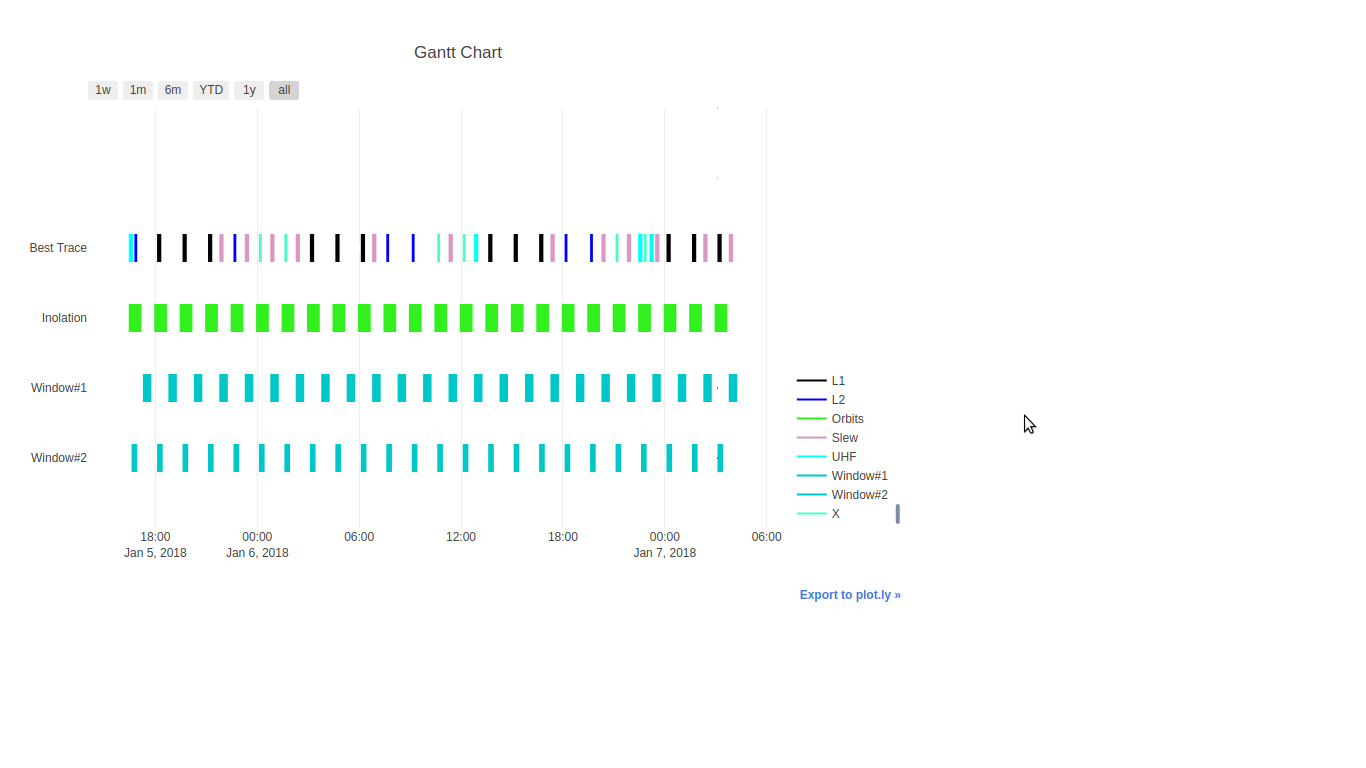
\includegraphics[width=\textwidth]{graphics/gantt.png}
	\caption{Graphical representation of the \gls{cora} schedule}
	\label{fig:gantt}
\end{figure}
